% !TeX root = ../phd-1st-year-presentation.tex
% !TeX encoding = UTF-8
% !TeX spellcheck = en_GB

\section{Analysis of assembly lines}
  \subsection{Assembly lines}
    \begin{frame}{Assembly line}
      \begin{center}\scalebox{0.9}{\tikzstyle{block} = [rectangle, draw, rounded corners, minimum height=2.5em, align=center, fill=white]
\tikzstyle{line} = [draw, -latex', line width=.3mm]

\begin{tikzpicture}[node distance = 1.5em, auto]
  % Place nodes
  \node [text width=1cm, align=center] at (0,0) (arrival) {\textit{product\\arrival}};
  \node [right = of arrival, block, square] (ws1) {$\pl{WS}_1$};
  \node [right = of ws1, block, square] (ws2) {$\pl{WS}_2$};
  \node [right = of ws2] (dots1) {\ldots};
  \node [right = of dots1, block, square] (wsk) {$\pl{WS}_{k}$};
  \node [right = of wsk] (dots2) {\ldots};
  \node [right = of dots2, block, square] (wsN) {$\pl{WS}_{N}$};
  \node [right = of wsN, text width=1.5cm, align=center] (production) {\textit{production\\complete}};
  % Draw edges
  \path [line] (arrival) -- (ws1);
  \path [line] (ws1) -- (ws2);
  \path [line] (ws2) -- (dots1);
  \path [line] (dots1) -- (wsk);
  \path [line] (wsk) -- (dots2);
  \path [line] (dots2) -- (wsN);
  \path [line] (wsN) -- (production);
\end{tikzpicture}}\end{center}
      
      \vspace{1em}
      \begin{minipage}{0.6\textwidth}
        $N$ sequential workstations $\pl{WS}_1, \dots, \pl{WS}_N$
        \begin{itemize}
          \item with transfer blocking
          \item and no buffering capacity
        \end{itemize}
        
        \vspace{1em}
        Workstation $\pl{WS_k}$ can be in one of three states
        \begin{itemize}
          \item \textit{producing}: $\pl{WS_k}$ is working on a product
          \item \textit{done}: $\pl{WS_k}$ is done working on a product
          \item \textit{idling}: $\pl{WS_k}$ is waiting for a new product
        \end{itemize}
      \end{minipage}
      \begin{minipage}{0.35\textwidth}
        \begin{center}\scalebox{0.8}{%Components styles
\tikzstyle{component state}=[draw, ellipse, minimum height = 0.5cm, minimum width = 2cm, thick, fill=white]
\tikzstyle{arc label}=[draw, align=left, fill=white, font={\scriptsize, \itshape}]
\tikzstyle{line} = [draw, -latex']

\begin{tikzpicture}
	%Workstation
	\node [component state] at (5,0) (WIdle) {idling};
	\node [component state] at (8,0) (WProducing) {producing};
	\node [component state] at (6.5,-2) (WDone) {done};
	
	\path [black,line,out=45,in=135] (WIdle) edge (WProducing);
	\path [black,line,out=270,in=0] (WProducing) edge (WDone);
	\path [black,line,out=180,in=270] (WDone) edge (WIdle);
	
	\node[arc label, align=center] at (6.5,1) {a product has arrived\\from workstation $\pl{WS}_{k-1}$};
	\node[arc label, align=center] at (8,-1.1) {production\\has finished};
	\node[arc label, align=center] at (5,-1.1) {workstation $\pl{WS}_{k+1}$\\has received\\the product};
\end{tikzpicture}}\end{center}
    \end{minipage}
    \end{frame}
    
    \begin{frame}{Workstation}
      Each workstation $\pl{WS}_k$
      \begin{itemize}
        \item has no internal parallelism
        \begin{itemize}
          \item at most one item being processed in each workstation
        \end{itemize}
        \item can implement complex workflows
        \begin{itemize}
          \item sequential/alternative/cyclic phases with random choices
        \end{itemize}
        \item and has GEN phases' durations
      \end{itemize}
      
      \begin{center}\scalebox{0.7}{\tikzstyle{decision} = [diamond, draw, node distance=3cm, inner sep=0pt, minimum height=3em, minimum width=3em, align=center, fill=white]
\tikzstyle{block} = [rectangle, draw, rounded corners, minimum height=2.5em, align=center, fill=white]
\tikzstyle{line} = [draw, -latex', line width=.3mm]

\begin{tikzpicture}[node distance = 1.5em, auto]
  \draw [black!25, line width=.5mm, rounded corners=1.75ex, fill=black!5] (0,0) rectangle (10.2,4) node[fitting node] (ws) {};
  \node [right = 2.5em of ws.north west, rectangle, draw, color=black!25, line width=.5mm, fill=white, text=black, rounded corners, minimum width=4em, minimum height=2em] (ws-name) {$\pl{WS}_k$};
  % Place nodes
  \node [above right = 6em and 1.5em of ws.south west, block, square] (p1) {$\pl{p}_1$};
  \node [left = 5em of p1] (wsk-1) {};
  \node [right = of p1, block, square] (p2) {$\pl{p}_2$};
  \node [right = of p2, decision] (s1) {$\pl{s}_1$};
  \node [above right = of s1, block, square] (p3a) {$\pl{p}_{3a}$};
  \node [below right = of s1, block, square] (p3b) {$\pl{p}_{3b}$};
  \node [right = of p3a, block, square] (p4a) {$\pl{p}_{4a}$};
  \node [right = of p3b, block, square] (p4b) {$\pl{p}_{4b}$};
  \node [right = of p4b, decision] (s2) {$\pl{s}_2$};
  \node [above right = of s2, block, square] (p5) {$\pl{p}_5$};
  \node [right = of p5, block, square] (d) {$\pl{d}$};
  \node [right = 5em of d] (wsk+1) {};
  % Draw edges
  \path [line] (wsk-1) -- (p1);
  \path [line] (p1) -- (p2);
  \path [line] (p2) -- (s1);
  \path [line] (s1) |- (p3a);
  \path [line] (s1) |- (p3b);
  \path [line] (p3a) -- (p4a);
  \path [line] (p3b) -- (p4b);
  \path [line] (p4b) -- (s2);
  \path [line] (s2) -- ++(0,-0.8) -| (p3b);
  \path [line] (p4a) -| (p5);
  \path [line] (s2) -| (p5);
  \path [line] (p5) -- (d);
  \path [line] (d) -- (wsk+1);
\end{tikzpicture}}\end{center}
      
      The last phase has no duration and encodes the \textit{done} state
    \end{frame}
    
    \begin{frame}{Underlying stochastic process}
      The underlying stochastic process of each isolated workstation\\
      is a Semi Markov Process (SMP)
      \begin{itemize}
        \item due to GEN durations
        \item and the absence of internal parallelism
      \end{itemize}
      
      \vspace{1.5em}
      The whole assembly line finds a renewal in any case where
      \begin{itemize}
        \item every \textit{done} station is in a queue before a bottleneck
        \item and everything else is \textit{idling}
      \end{itemize}
      
      \begin{center}\scalebox{0.8}{\relaxnewsetlength{\nodewidth}{2.5em}
\relaxnewsetlength{\nodedistance}{1.5em}
\relaxnewsetlength{\workingnodewidth}{0.7\nodewidth}

\tikzstyle{block} = [rectangle, draw, rounded corners, minimum height=\nodewidth, align=center, fill=white]
\tikzstyle{line} = [draw, -latex', line width=.3mm]
\definecolor{notidlegray}{gray}{0.8}
\tikzstyle{notidle} = [fill=notidlegray]

\begin{tikzpicture}[node distance = \nodedistance, auto]
  % Place nodes
  \node [text width=1cm, align=center] at (0,0) (arrival) {\textit{arrival}};
  \node [right = of arrival, block, square] (ws1) {$\pl{WS}_1$};
  \node [right = of ws1, block, square, notidle] (ws2) {$\pl{WS}_{2}$};
  \node [right = of ws2, block, square, notidle] (ws3) {$\pl{WS}_{3}$};
  \node [right = of ws3, block, square] (ws4-white-background) {};
  \fill [notidlegray, draw] ($(ws4-white-background.north west) + (\workingnodewidth,0)$) {[rounded corners] -- ++(-\workingnodewidth,0) -- ++(0,-\nodewidth)} -- ++(\workingnodewidth,0) -- cycle {};
  \node [right = of ws3, block, square, fill=none] (ws4) {$\pl{WS}_{4}$};
  \node [right = of ws4, block, square] (ws5) {$\pl{WS}_{5}$};
  \node [right = of ws5, block, square] (ws6) {$\pl{WS}_{6}$};
  \node [right = of ws6, text width=1.5cm, align=center] (production) {\textit{completion}};
  % Draw edges
  \path [line] (arrival) -- (ws1);
  \path [line] (ws1) -- (ws2);
  \path [line] (ws2) -- (ws3);
  \path [line] (ws3) -- (ws4);
  \path [line] (ws4) -- (ws5);
  \path [line] (ws5) -- (ws6);
  \path [line] (ws6) -- (production);
\end{tikzpicture}}\end{center}
    \end{frame}
  
  \subsection{Inspection}
    \begin{frame}{Inspection with partial observability}
      
      The assembly line can be inspected by external observers
      \begin{itemize}
        \item the line can be considered at steady-state at inspection
        \item there can be ambiguity about the current phase
      \end{itemize}
      
      \vspace{1em}
      An observation is a tuple $\omega=\langle \omega_0, \omega_1,\ldots, \omega_N \rangle$
      \begin{itemize}
        \item $\omega_0$ indicates if a new product is ready to enter the line or not
        \item $\omega_k = \langle \sigma_k, \phi_k \rangle$ refers to $\pl{WS}_k$
        \begin{itemize}
          \item $\sigma_k$ indicates if $\pl{WS}_k$ is \textit{idle}/\textit{producing}/\textit{done}
          \item $\phi_k$ identifies the set of possible current phases
        \end{itemize}
      \end{itemize}
        
      \vspace{1em}
      \begin{minipage}{0.65\textwidth}
        Two kinds of uncertainty
        \begin{itemize}
          \item about the actual current phase
          \begin{itemize}
            \item discrete
          \end{itemize}
          \item about the remaining time in the current phase%
          \begin{itemize}
            \item continuous
          \end{itemize}
        \end{itemize}
      \end{minipage}
      \begin{minipage}{0.3\textwidth}
        \begin{center}\scalebox{0.65}{\let\observationdistance\relax
\newlength{\observationdistance}
\setlength{\observationdistance}{0.1em}

\tikzstyle{decision} = [diamond, draw, node distance=3cm, inner sep=0pt, minimum height=3em, minimum width=3em, align=center, fill=white]
\tikzstyle{block} = [rectangle, draw, rounded corners, minimum height=2.5em, align=center, fill=white]
\tikzstyle{line} = [draw, -latex', line width=.3mm]

\tikzstyle{north-east-lines} = [preaction={fill, white}, pattern=north east lines, pattern color=black!30]

\begin{tikzpicture}[node distance = 1.5em, auto]
  \draw [black!25, line width=.5mm, rounded corners=1.75ex, fill=black!5] (0,0) rectangle (5.1,3.7) node[fitting node] (ws) {};
  \node [right = 1em of ws.north west, rectangle, draw, color=black!25, line width=.5mm, fill=white, text=black, rounded corners, minimum width=2em, minimum height=1.5em] (ws-name) {$\pl{WK}_{k}$};
  % Place nodes
  \node [above right = 4.3em and 1.5em of ws.south west, block, square, fill=black!25] (p1) {$\pl{p}_1$};
  \node [above = \observationdistance of p1] (p1-obs) {$o_1$};
  \node [left = 3em of p1] (wsk-1) {};
  \node [right = of p1, decision] (s1) {$\pl{s}_1$};
  \node [above right = of s1, block, square, north-east-lines] (p2a) {$\pl{p}_{2a}$};
  \node [above = \observationdistance of p2a] (p2a-obs) {$o_2$};
  \node [below right = of s1, block, square, north-east-lines] (p2b) {$\pl{p}_{2b}$};
  \node [above = \observationdistance of p2b] (p2b-obs) {$o_2$};
  \node [below right = of p2a, block, square] (d) {$\pl{d}$};
  \node [right = 3em of d] (wsk+1) {};
  % Draw edges
  \path [line] (wsk-1) -- (p1);
  \path [line] (p1) -- (s1);
  \path [line] (s1) |- (p2a);
  \path [line] (s1) |- (p2b);
  \path [line] (p2a) -| (d);
  \path [line] (p2b) -| (d);
  \path [line] (d) -- (wsk+1);
\end{tikzpicture}}\end{center}
      \end{minipage}
    \end{frame}
  
  \subsection{Performance measures}
    \begin{frame}{Performance measures}
      \relaxnewsetlength{\descriptionwidth}{0.6\textwidth}
      \relaxnewsetlength{\schemawidth}{0.35\textwidth}
      \newcommand{\schemascale}{0.45}
      \relaxnewsetlength{\vspacegap}{1.5em}
      
      \begin{minipage}{\descriptionwidth}
        \textbf{Time To Done}
        \begin{itemize}
          \item The remaining time until workstation $k$,\\
            according to observation $\omega$,\\
            reaches the \textit{done} state
        \end{itemize}
      \end{minipage}
      \begin{minipage}{\schemawidth}
        \begin{center}\scalebox{\schemascale}{%Components styles
\tikzstyle{component state}=[draw, ellipse, minimum height = 0.5cm, minimum width = 2cm, thick, fill=white]
\tikzstyle{arc label}=[draw, align=left, fill=white, font={\scriptsize, \itshape}]
\tikzstyle{line} = [draw, -latex']

\begin{tikzpicture}
	%Workstation
	\node [component state] at (5,0) (WIdle) {idling};
	\node [component state] at (8,0) (WProducing) {producing};
	\node [component state, fill=black!25] at (6.5,-2) (WDone) {done};
	
	\path [black,line,out=45,in=135] (WIdle) edge (WProducing);
	\path [black,line,out=270,in=0] (WProducing) edge (WDone);
	\path [black,line,out=180,in=270] (WDone) edge (WIdle);
	
	\node[arc label, align=center] at (6.5,1) {a product has arrived\\from workstation $\pl{WS}_{k-1}$};
	\node[arc label, align=center] at (8,-1.1) {production\\has finished};
	\node[arc label, align=center] at (5,-1.1) {workstation $\pl{WS}_{k+1}$\\has received\\the product};
\end{tikzpicture}}\end{center}
      \end{minipage}

      \vspace{\vspacegap}
      \begin{minipage}{\descriptionwidth}
        \textbf{Time To Idle}
        \begin{itemize}
          \item The remaining time until workstation $k$,\\
            according to observation $\omega$,\\
            reaches the \textit{idling} state
        \end{itemize}
      \end{minipage}
      \begin{minipage}{\schemawidth}
        \begin{center}\scalebox{\schemascale}{%Components styles
\tikzstyle{component state}=[draw, ellipse, minimum height = 0.5cm, minimum width = 2cm, thick, fill=white]
\tikzstyle{arc label}=[draw, align=left, fill=white, font={\scriptsize, \itshape}]
\tikzstyle{line} = [draw, -latex']

\begin{tikzpicture}
	%Workstation
	\node [component state, fill=black!25] at (5,0) (WIdle) {idling};
	\node [component state] at (8,0) (WProducing) {producing};
	\node [component state] at (6.5,-2) (WDone) {done};
	
	\path [black,line,out=45,in=135] (WIdle) edge (WProducing);
	\path [black,line,out=270,in=0] (WProducing) edge (WDone);
	\path [black,line,out=180,in=270] (WDone) edge (WIdle);
	
	\node[arc label, align=center] at (6.5,1) {a product has arrived\\from workstation $\pl{WS}_{k-1}$};
	\node[arc label, align=center] at (8,-1.1) {production\\has finished};
	\node[arc label, align=center] at (5,-1.1) {workstation $\pl{WS}_{k+1}$\\has received\\the product};
\end{tikzpicture}}\end{center}
      \end{minipage}
      
      \vspace{\vspacegap}
      \begin{minipage}{\descriptionwidth}
        \textbf{Time To Start Next}
        \begin{itemize}
          \item The remaining time until workstation $k$,\\
            according to observation $\omega$,\\
            starts the production of a new product
        \end{itemize}
      \end{minipage}
      \begin{minipage}{\schemawidth}
        \begin{center}\scalebox{\schemascale}{%Components styles
\tikzstyle{component state}=[draw, ellipse, minimum height = 0.5cm, minimum width = 2cm, thick, fill=white]
\tikzstyle{arc label}=[draw, align=left, fill=white, font={\scriptsize, \itshape}]
\tikzstyle{line} = [draw, -latex']

\begin{tikzpicture}
	%Workstation
	\node [component state] at (5,0) (WIdle) {idling};
	\node [component state] at (8,0) (WProducing) {producing};
	\node [component state] at (6.5,-2) (WDone) {done};
	
	\path [black,line,out=45,in=135] (WIdle) edge (WProducing);
	\path [black,line,out=270,in=0] (WProducing) edge (WDone);
	\path [black,line,out=180,in=270] (WDone) edge (WIdle);
	
	\node[arc label, align=center, fill=black!25] at (6.5,1) {a product has arrived\\from workstation $\pl{WS}_{k-1}$};
	\node[arc label, align=center] at (8,-1.1) {production\\has finished};
	\node[arc label, align=center] at (5,-1.1) {workstation $\pl{WS}_{k+1}$\\has received\\the product};
\end{tikzpicture}}\end{center}
      \end{minipage}
    \end{frame}
     
  \subsection{Evaluation of performance measures}
    \begin{frame}{Time To Done}
      \begin{equation*}
        \mbox{TTD}(k,\omega) := \left\{ \begin{array}{ll}
          \displaystyle \sum_{\gamma\in \phi_k} P_{k, \gamma,\omega} \cdot (R(k,\gamma) + Z(k,\gamma)), &  \mbox{ if } \sigma_k=\mbox{\em producing}
          \medskip\\
          \mbox{TTD}(k-1,\omega) + V(k), & \mbox{ if } \sigma_k=\mbox{\em idling}
          \medskip\\
          0, & \mbox{ if } \sigma_k=\mbox{\em done}
        \end{array} \right.
        \label{eq:ttd}
      \end{equation*}
      
      \begin{itemize}
        \item $P_{k,\gamma,\omega}$ probability weight that $\pl{WS}_k$ is in phase $\gamma$ according to $\omega$
        \item $R(k,\gamma)$ \textit{remaining time} in phase $\gamma$ of $\pl{WS}_k$
        \item $Z(k,\gamma)$ \textit{execution time} of phases of $\pl{WS}_k$ that follow $\gamma$
        \item $V(k)$ \textit{production time} of $\pl{WS}_k$
      \end{itemize}
      
      \begin{center}\hspace{-0.5cm}\scalebox{0.8}{\relaxnewsetlength{\nodewidth}{2.5em}
\relaxnewsetlength{\nodedistance}{1.5em}
\relaxnewsetlength{\workingnodewidth}{0.7\nodewidth}

\relaxnewsetlength{\nodemeasuredistance}{0.15em}
\relaxnewsetlength{\pathopdistance}{1.4em}

\tikzstyle{block} = [rectangle, draw, rounded corners, minimum height=\nodewidth, align=center, fill=white]
\tikzstyle{line} = [draw, -latex', line width=.3mm]
\definecolor{notidlegray}{gray}{0.8}
\tikzstyle{notidle} = [fill=notidlegray]

\begin{tikzpicture}[node distance = \nodedistance, auto]
  % Place nodes
  \node [text width=1cm, align=center] at (0,0) (arrival) {\textit{arrival}};
  
  \node [right = of arrival, block, square] (ws1-white-background) {};
  \fill [notidlegray, draw] ($(ws1-white-background.north west) + (\workingnodewidth,0)$) {[rounded corners] -- ++(-\workingnodewidth,0) -- ++(0,-\nodewidth)} -- ++(\workingnodewidth,0) -- cycle {};
  \node [right = of arrival, block, square, fill=none] (ws1) {$\pl{WS}_{1}$};
  \node [below = \nodemeasuredistance of ws1, align=center] (ws1-measure) {$\scriptstyle(R_1+Z_1)$};
  
  \node [right = of ws1, block, square] (ws2) {$\pl{WS}_{2}$};
  \node [below = \nodemeasuredistance of ws2, align=center] (ws2-measure) {$\scriptstyle V_2$};
  
  \node [right = of ws2, block, square] (ws3) {$\pl{WS}_{3}$};
  \node [below = \nodemeasuredistance of ws3, align=center] (ws3-measure) {$\scriptstyle V_3$};
  \node [above = \nodemeasuredistance of ws3, align=center] (TTD3) {$\scriptstyle TTD_3$};
  
  \node [right = of ws3, block, square, notidle] (ws4) {$\pl{WS}_{4}$};
  
  \node [right = of ws4, block, square] (ws5-white-background) {};
  \fill [notidlegray, draw] ($(ws5-white-background.north west) + (\workingnodewidth,0)$) {[rounded corners] -- ++(-\workingnodewidth,0) -- ++(0,-\nodewidth)} -- ++(\workingnodewidth,0) -- cycle {};
  \node [right = of ws4, block, square, fill=none] (ws5) {$\pl{WS}_{5}$};
  
  \node [right = of ws5, block, square] (ws6-white-background) {};
  \fill [notidlegray, draw] ($(ws6-white-background.north west) + (\workingnodewidth,0)$) {[rounded corners] -- ++(-\workingnodewidth,0) -- ++(0,-\nodewidth)} -- ++(\workingnodewidth,0) -- cycle {};
  \node [right = of ws5, block, square, fill=none] (ws6) {$\pl{WS}_{6}$};
  
  \node [right = of ws6, text width=1.5cm, align=center] (production) {\textit{completion}};
  % Draw edges
  \path [line] (arrival) -- (ws1);
  \path [line] (ws1) -- coordinate[midway] (ws1ws2) (ws2);
  \node [below = \pathopdistance of ws1ws2, align=center] (ws1ws2-op) {$\scriptstyle+$};
  \path [line] (ws2) -- coordinate[midway] (ws2ws3) (ws3);
  \node [below = \pathopdistance of ws2ws3, align=center] (ws2ws3-op) {$\scriptstyle+$};
  \path [line] (ws3) -- (ws4);
  \path [line] (ws4) -- (ws5);
  \path [line] (ws5) -- (ws6);
  \path [line] (ws6) -- (production);
\end{tikzpicture}}\end{center}
      
      Backward recursive evaluation
    \end{frame}
    
    \begin{frame}{Time To Idle}
      \begin{equation*}
        \mbox{TTI}(k,\omega) := \left\{ \begin{array}{ll}
          \max\{\mbox{TTD}(k,\omega),\mbox{TTI}(k+1,\omega)\}, & \mbox{ if } \sigma_k\in\{\mbox{\em producing}, \mbox{\em done}\}
          \medskip\\
          0, & \mbox{ if } \sigma_k=\mbox{\em idling}
        \end{array} \right.
        \label{eq:tti}
      \end{equation*}
      
      \begin{itemize}
        \item $\mbox{TTI}(k,\omega)=\max\{ \mbox{TTD}(k,\omega), \ldots, \mbox{TTD}(k+n,\omega) \}$
        \begin{itemize}
          \item $\pl{WS}_j$ producing/done $\forall j \in [k,k+n]$
          \item either $\pl{WS}_{k+n}$ last workstation or $\pl{WS}_{k+n+1}$ idling
        \end{itemize}
        \item $\pl{WS}_k$ becomes idle when the bottleneck finishes its production
      \end{itemize}
      
      \begin{center}\hspace{-1.5cm}\scalebox{0.8}{\relaxnewsetlength{\nodewidth}{2.5em}
\relaxnewsetlength{\nodedistance}{1.5em}
\relaxnewsetlength{\workingnodewidth}{0.7\nodewidth}

\relaxnewsetlength{\nodemeasuredistance}{0.15em}
\relaxnewsetlength{\pathopdistance}{1.4em}
\relaxnewsetlength{\extradistance}{0.25em}
\relaxnewsetlength{\nodemeasuredistanceextra}{\nodemeasuredistance + \extradistance}
\relaxnewsetlength{\pathopdistanceextra}{\pathopdistance + \extradistance + 0.2em}

\tikzstyle{block} = [rectangle, draw, rounded corners, minimum height=\nodewidth, align=center, fill=white]
\tikzstyle{line} = [draw, -latex', line width=.3mm]
\definecolor{notidlegray}{gray}{0.8}
\tikzstyle{notidle} = [fill=notidlegray]

\begin{tikzpicture}[node distance = \nodedistance, auto]
  % Place nodes
  \node [text width=1cm, align=center] at (0,0) (arrival) {\textit{arrival}};
  
  \node [right = of arrival, block, square] (ws1-white-background) {};
  \fill [notidlegray, draw] ($(ws1-white-background.north west) + (\workingnodewidth,0)$) {[rounded corners] -- ++(-\workingnodewidth,0) -- ++(0,-\nodewidth)} -- ++(\workingnodewidth,0) -- cycle {};
  \node [right = of arrival, block, square, fill=none] (ws1) {$\pl{WS}_{1}$};
  
  \node [right = of ws1, block, square] (ws2) {$\pl{WS}_{2}$};
  
  \node [right = of ws2, block, square] (ws3) {$\pl{WS}_{3}$};
  
  \node [right = of ws3, block, square, notidle] (ws4) {$\pl{WS}_{4}$};
  \node [below = \nodemeasuredistance of ws4, align=center] (ws4-measure) {$(\scriptstyle 0,$};
  \node [above = \nodemeasuredistance of ws4, align=center] (TTI4) {$\scriptstyle TTI_4$};
  
  \node [right = of ws4, block, square] (ws5-white-background) {};
  \fill [notidlegray, draw] ($(ws5-white-background.north west) + (\workingnodewidth,0)$) {[rounded corners] -- ++(-\workingnodewidth,0) -- ++(0,-\nodewidth)} -- ++(\workingnodewidth,0) -- cycle {};
  \node [right = of ws4, block, square, fill=none] (ws5) {$\pl{WS}_{5}$};
  \node [below = \nodemeasuredistanceextra of ws5, align=center] (ws5-measure) {$\scriptstyle (R_5+Z_5),$};
  
  \node [right = of ws5, block, square] (ws6-white-background) {};
  \fill [notidlegray, draw] ($(ws6-white-background.north west) + (\workingnodewidth,0)$) {[rounded corners] -- ++(-\workingnodewidth,0) -- ++(0,-\nodewidth)} -- ++(\workingnodewidth,0) -- cycle {};
  \node [right = of ws5, block, square, fill=none] (ws6) {$\pl{WS}_{6}$};
  \node [below = \nodemeasuredistance of ws6, align=center] (ws6-measure) {${\scriptstyle (R_6+Z_6)})$};
  
  \node [right = of ws6, text width=1.5cm, align=center] (production) {\textit{completion}};
  % Draw edges
  \path [line] (arrival) -- (ws1);
  \path [line] (ws1) -- (ws2);
  \path [line] (ws2) -- (ws3);
  \path [line] (ws3) -- coordinate[midway] (ws3ws4)  (ws4);
  \node [below right = \pathopdistanceextra and -0.2em of ws3ws4, align=center] (ws3ws4-op) {$\scriptstyle\max$};
  \path [line] (ws4) -- (ws5);
  \path [line] (ws5) -- (ws6);
  \path [line] (ws6) -- (production);
\end{tikzpicture}}\end{center}
      
      Forward recursive evaluation
    \end{frame}
    
    \begin{frame}{Time To Start Next}
      \begin{equation*}
        \mbox{TTSN}(k,\omega) := \max\{ \mbox{TTI}(k,\omega), \mbox{TTD}(k-1,\omega) \}
        \label{eq:ttn}
      \end{equation*}
      
      \vspace{1em}
      \begin{center}\hspace{-1.5cm}\scalebox{0.8}{\relaxnewsetlength{\nodewidth}{2.5em}
\relaxnewsetlength{\nodedistance}{1.5em}
\relaxnewsetlength{\workingnodewidth}{0.7\nodewidth}

\relaxnewsetlength{\nodemeasuredistance}{0.15em}
\relaxnewsetlength{\pathopdistance}{1.4em}
\relaxnewsetlength{\extradistance}{0.3em}
\relaxnewsetlength{\nodemeasuredistanceextra}{\nodemeasuredistance + \extradistance}
\relaxnewsetlength{\pathopdistanceextra}{\pathopdistance + \extradistance}

\tikzstyle{block} = [rectangle, draw, rounded corners, minimum height=\nodewidth, align=center, fill=white]
\tikzstyle{line} = [draw, -latex', line width=.3mm]
\definecolor{notidlegray}{gray}{0.8}
\tikzstyle{notidle} = [fill=notidlegray]

\begin{tikzpicture}[node distance = \nodedistance, auto]
  % Place nodes
  \node [text width=1cm, align=center] at (0,0) (arrival) {\textit{arrival}};
  
  \node [right = of arrival, block, square] (ws1-white-background) {};
  \fill [notidlegray, draw] ($(ws1-white-background.north west) + (\workingnodewidth,0)$) {[rounded corners] -- ++(-\workingnodewidth,0) -- ++(0,-\nodewidth)} -- ++(\workingnodewidth,0) -- cycle {};
  \node [right = of arrival, block, square, fill=none] (ws1) {$\pl{WS}_{1}$};
  \node [below = \nodemeasuredistance of ws1, align=center] (ws1-measure) {$(\scriptstyle(R_1+Z_1)$};
  
  \node [right = of ws1, block, square] (ws2) {$\pl{WS}_{2}$};
  \node [below = \nodemeasuredistanceextra of ws2, align=center] (ws2-measure) {$\scriptstyle V_2$};
  
  \node [right = of ws2, block, square] (ws3) {$\pl{WS}_{3}$};
  \node [below = \nodemeasuredistance of ws3, align=center] (ws3-measure) {${\scriptstyle V_3}),$};
  
  \node [right = of ws3, block, square, notidle] (ws4) {$\pl{WS}_{4}$};
  \node [below = \nodemeasuredistanceextra of ws4, align=center] (ws4-measure) {$\scriptstyle 0,$};
  \node [above = \nodemeasuredistance of ws4, align=center] (TTI4) {$\scriptstyle TTSN_4$};
  
  \node [right = of ws4, block, square] (ws5-white-background) {};
  \fill [notidlegray, draw] ($(ws5-white-background.north west) + (\workingnodewidth,0)$) {[rounded corners] -- ++(-\workingnodewidth,0) -- ++(0,-\nodewidth)} -- ++(\workingnodewidth,0) -- cycle {};
  \node [right = of ws4, block, square, fill=none] (ws5) {$\pl{WS}_{5}$};
  \node [below = \nodemeasuredistanceextra of ws5, align=center] (ws5-measure) {$\scriptstyle (R_5+Z_5),$};
  
  \node [right = of ws5, block, square] (ws6-white-background) {};
  \fill [notidlegray, draw] ($(ws6-white-background.north west) + (\workingnodewidth,0)$) {[rounded corners] -- ++(-\workingnodewidth,0) -- ++(0,-\nodewidth)} -- ++(\workingnodewidth,0) -- cycle {};
  \node [right = of ws5, block, square, fill=none] (ws6) {$\pl{WS}_{6}$};
  \node [below = \nodemeasuredistance of ws6, align=center] (ws6-measure) {${\scriptstyle (R_6+Z_6)}))$};
  
  \node [right = of ws6, text width=1.5cm, align=center] (production) {\textit{completion}};
  % Draw edges
  \path [line] (arrival) -- coordinate[midway] (arrivalws1) (ws1);
  \node [below right = \pathopdistance and -1.5em of arrivalws1, align=center] (arrivalws1-op) {${\scriptstyle\max}($};
  \path [line] (ws1) -- coordinate[midway] (ws1ws2) (ws2);
  \node [below = \pathopdistanceextra of ws1ws2, align=center] (ws1ws2-op) {$\scriptstyle+$};
  \path [line] (ws2) -- coordinate[midway] (ws2ws3) (ws3);
  \node [below = \pathopdistanceextra of ws2ws3, align=center] (ws2ws3-op) {$\scriptstyle+$};
  \path [line] (ws3) -- coordinate[midway] (ws3ws4)  (ws4);
  \node [below right = \pathopdistance and -0.4em of ws3ws4, align=center] (ws3ws4-op) {${\scriptstyle\max}($};
  \path [line] (ws4) -- (ws5);
  \path [line] (ws5) -- (ws6);
  \path [line] (ws6) -- (production);
\end{tikzpicture}}\end{center}
      
      Forward and backward recursive evaluation
    \end{frame}
    
    \begin{frame}{Disambiguation of observed phases}
      Resolve observed (producing) phases' ambiguity
      \begin{itemize}
        \item steady-state probability that $\pl{WS}_k$ is in phase $\gamma$ according to $\omega$
      \end{itemize}
      Given observation $\phi_k$ for workstation $\pl{WS}_k$
      \begin{itemize}
        \item we compute probability $P_{k,\gamma,\omega}$
        \item that it was actually $\gamma$ that produced $\phi_k$
      \end{itemize}
      
     	\begin{equation*}
       	P_{k,\gamma,\omega} = \frac{\tilde{\pi}(\gamma)}{\displaystyle \sum_{\gamma' \in \phi_k} \tilde{\pi}(\gamma')}
       	\label{eq:probabilityObservation}
     	\end{equation*}
     	
     	\begin{itemize}
       	\item $\tilde{\pi}(\gamma)$ steady-state probability of phase $\gamma$ in an isolated model of $\pl{WS}_k$
     	\end{itemize}
    \end{frame}
    
    \begin{frame}{Isolated workstation model}
      The isolated workstation model represents a workstation\\
      repeatedly processing a product
      \begin{itemize}
        \item one product being processed
        \item after its production, it's moved back to the entry point of the workstation
      \end{itemize}
      
      \begin{center}\scalebox{0.6}{\tikzstyle{decision} = [diamond, draw, node distance=3cm, inner sep=0pt, minimum height=3em, minimum width=3em, align=center, fill=white]
\tikzstyle{block} = [rectangle, draw, rounded corners, minimum height=2.5em, align=center, fill=white]
\tikzstyle{line} = [draw, -latex', line width=.3mm]

\begin{tikzpicture}[node distance = 1.5em, auto]
  \draw [black!25, line width=.5mm, rounded corners=1.75ex, fill=black!5] (0,0) rectangle (10.2,4) node[fitting node] (ws) {};
  \node [right = 2.5em of ws.north west, rectangle, draw, color=black!25, line width=.5mm, fill=white, text=black, rounded corners, minimum width=4em, minimum height=2em] (ws-name) {$\pl{WS}_k$};
  % Place nodes
  \node [above right = 6em and 1.5em of ws.south west, block, square] (p1) {$\pl{p}_1$};
  \node [right = of p1, block, square] (p2) {$\pl{p}_2$};
  \node [right = of p2, decision] (s1) {$\pl{s}_1$};
  \node [above right = of s1, block, square] (p3a) {$\pl{p}_{3a}$};
  \node [below right = of s1, block, square] (p3b) {$\pl{p}_{3b}$};
  \node [right = of p3a, block, square] (p4a) {$\pl{p}_{4a}$};
  \node [right = of p3b, block, square] (p4b) {$\pl{p}_{4b}$};
  \node [right = of p4b, decision] (s2) {$\pl{s}_2$};
  \node [above right = of s2, block, square] (p5) {$\pl{p}_5$};
  \node [right = of p5, block, square] (d) {$\pl{d}$};
  % Draw edges
  \path [line] (p1) -- (p2);
  \path [line] (p2) -- (s1);
  \path [line] (s1) |- (p3a);
  \path [line] (s1) |- (p3b);
  \path [line] (p3a) -- (p4a);
  \path [line] (p3b) -- (p4b);
  \path [line] (p4b) -- (s2);
  \path [line] (s2) -- ++(0,-0.8) -| (p3b);
  \path [line] (p4a) -| (p5);
  \path [line] (s2) -| (p5);
  \path [line] (p5) -- (d);
  \path [line] (d) -- ++(5em,0) -- ++(0,2.5) -- ($(p1) + (-5em,2.5)$) -- ($(p1) + (-5em,0)$) -- (p1);
\end{tikzpicture}}\end{center}
      
      It can be used for two reasons
      \begin{itemize}
        \item steady-state probabilities of producing phases are independent
        \item the inspection is at steady-state
        \begin{itemize}
          \item arrivals and productions can be considerer in equilibrium
        \end{itemize}
      \end{itemize}
    \end{frame}
    
    \begin{frame}{Remaining time}
      Evaluation of $F_{R(k,\gamma)}(t) = $ CDF of $R(k,\gamma)$
      \begin{itemize}
        \item $R(k,\gamma)$ \textit{remaining time} in phase $\gamma$ of $\pl{WS}_k$
      \end{itemize}
      
      \vspace{1em}
      Problem!
      \begin{itemize}
        \item remaining times of enabled GEN transitions are \textit{dependent}
        \item joint probabilities don't allow for a compositional approach
      \end{itemize}
      
      \vspace{1em}
      $\sfrac{1}{3}$ \textit{Immediate} approximation
      \begin{itemize}
        \item assume that phase $\gamma$ is inspected at its ending
        \begin{itemize}
          \item $\tilde{F}_{R(k, \gamma)}(t) = 1 \quad \forall t$
        \end{itemize}
        \item represents an \textit{upper bound}
      \end{itemize}
      
      \vspace{1em}
      $\sfrac{2}{3}$ \textit{Newly enabled} approximation
      \begin{itemize}
        \item assume that phase $\gamma$ is inspected at its beginning
        \begin{itemize}
          \item $\tilde{F}_{R(k, \gamma)}(t) = F_{\gamma}(t)$ 
          \item $F_{\gamma}(t)$ original CDF of the duration of $\gamma$
        \end{itemize}
        \item represents a \textit{lower bound}
      \end{itemize}
    \end{frame}
    
    \begin{frame}{Remaining time}
      $\sfrac{3}{3}$ \textit{Independent remaining times} approximation
      \begin{itemize}
        \item consider the remaining times of ongoing phases as \textit{independent}
        \item represents a (better) \textit{lower bound}
      \end{itemize}
      
      \begin{block}{Theorem: positive correlation \& stochastic order}
        If $\hat{R}$ is an independent version of vector $R$ of positively correlated remaining times of ongoing phases, then $\hat{R} \geq_{st} R$
      \end{block}
      
      \vspace{1em}
      Steady-state distribution of $\hat{R}(k,\gamma)$\\
      computed according to the Key Renewal Theorem\footnote{\scriptsize Serfozo, R., 2009. Basics of applied stochastic processes. Springer Science \& Business Media.}
      \begin{equation*}
        \tilde{F}_{R(k,\gamma)}(t) = \frac{1}{\mu} \int_{0}^{t} [1 - F_{\gamma}(s)]ds
      \end{equation*}
      \begin{itemize}
        \item $\mu$ expected value of $F_{\gamma}(t)$
      \end{itemize}
    \end{frame}
    
    \begin{frame}{Execution and production time}
      Evaluation of $F_{Z(k,\gamma)}(t)$ and $F_{V(k)}$
      \begin{itemize}
        \item $Z(k,\gamma)$ \textit{execution time} of phases of $\pl{WS}_k$ that follow $\gamma$
        \item $V(k)$ \textit{production time} of $\pl{WS}_k$
      \end{itemize}
    
      \vspace{1em}
      CDFs of $Z(k,\gamma)$ and $V(k)$ are computed as transient probabilities
      
      \begin{itemize}
        \item $F_{Z(k,\gamma)}$ transient probability from phase after $\gamma$ to final phase of $\pl{WS}_k$
        \item $F_{V(k)}$ transient probability from first phase to final phase of $\pl{WS}_k$
      \end{itemize}
      
      \vspace{2em}
      Upper/lower bounds for \textit{TTD}, \textit{TTI} and \textit{TTSN} can be evaluated
      \begin{itemize}
        \item \textit{convolution} and \textit{max} operations maintain stochastic order
      \end{itemize}
    \end{frame}
    
  \subsection{Experimentation}
    \begin{frame}{Case study assembly lines}
      Sequential, alternative and cyclic workstations
      
      \vspace{0.5em}
      \begin{minipage}{0.3\textwidth}
        \begin{center}\scalebox{0.5}{\let\observationdistance\relax
\newlength{\observationdistance}
\setlength{\observationdistance}{0.1em}

\tikzstyle{block} = [rectangle, draw, rounded corners, minimum height=2.5em, align=center, fill=white]
\tikzstyle{line} = [draw, -latex', line width=.3mm]

\tikzstyle{north-east-lines} = [preaction={fill, white}, pattern=north east lines, pattern color=black!30]

\begin{tikzpicture}[node distance = 1.5em, auto]
  \draw [black!25, line width=.5mm, rounded corners=1.75ex, fill=black!5] (0,0) rectangle (4.2,2) node[fitting node] (ws) {};
  \node [right = 1em of ws.north west, rectangle, draw, color=black!25, line width=.5mm, fill=white, text=black, rounded corners, minimum width=2em, minimum height=1.5em] (ws-name) {$\pl{sequential}$};
  % Place nodes
  \node [above right = 1.6em and 1.5em of ws.south west, block, square, fill=black!25] (p1) {$\pl{p}_1$};
  \node [above = \observationdistance of p1] (p1-obs) {$o_1$};
  \node [left = 3em of p1] (wsk-1) {};
  \node [right = of p1, block, square, north-east-lines] (p2) {$\pl{p}_2$};
  \node [above = \observationdistance of p2] (p2-obs) {$o_2$};
  \node [right = of p2, block, square] (d) {$\pl{d}$};
  \node [right = 3em of d] (wsk+1) {};
  % Draw edges
  \path [line] (wsk-1) -- (p1);
  \path [line] (p1) -- (p2);
  \path [line] (p2) -- (d);
  \path [line] (d) -- (wsk+1);
\end{tikzpicture}}\end{center}
      \end{minipage}
      \begin{minipage}{0.325\textwidth}
        \begin{center}\scalebox{0.5}{\let\observationdistance\relax
\newlength{\observationdistance}
\setlength{\observationdistance}{0.1em}

\tikzstyle{decision} = [diamond, draw, node distance=3cm, inner sep=0pt, minimum height=3em, minimum width=3em, align=center, fill=white]
\tikzstyle{block} = [rectangle, draw, rounded corners, minimum height=2.5em, align=center, fill=white]
\tikzstyle{line} = [draw, -latex', line width=.3mm]

\tikzstyle{north-east-lines} = [preaction={fill, white}, pattern=north east lines, pattern color=black!30]

\begin{tikzpicture}[node distance = 1.5em, auto]
  \draw [black!25, line width=.5mm, rounded corners=1.75ex, fill=black!5] (0,0) rectangle (5.1,3.7) node[fitting node] (ws) {};
  \node [right = 1em of ws.north west, rectangle, draw, color=black!25, line width=.5mm, fill=white, text=black, rounded corners, minimum width=2em, minimum height=1.5em] (ws-name) {$\pl{alternative}$};
  % Place nodes
  \node [above right = 4.3em and 1.5em of ws.south west, block, square, fill=black!25] (p1) {$\pl{p}_1$};
  \node [above = \observationdistance of p1] (p1-obs) {$o_1$};
  \node [left = 3em of p1] (wsk-1) {};
  \node [right = of p1, decision] (s1) {$\pl{s}_1$};
  \node [above right = of s1, block, square, north-east-lines] (p2a) {$\pl{p}_{2a}$};
  \node [above = \observationdistance of p2a] (p2a-obs) {$o_2$};
  \node [below right = of s1, block, square, north-east-lines] (p2b) {$\pl{p}_{2b}$};
  \node [above = \observationdistance of p2b] (p2b-obs) {$o_2$};
  \node [below right = of p2a, block, square] (d) {$\pl{d}$};
  \node [right = 3em of d] (wsk+1) {};
  % Draw edges
  \path [line] (wsk-1) -- (p1);
  \path [line] (p1) -- (s1);
  \path [line] (s1) |- (p2a);
  \path [line] (s1) |- (p2b);
  \path [line] (p2a) -| (d);
  \path [line] (p2b) -| (d);
  \path [line] (d) -- (wsk+1);
\end{tikzpicture}}\end{center}
      \end{minipage}
      \begin{minipage}{0.325\textwidth}
        \begin{center}\scalebox{0.5}{\let\observationdistance\relax
\newlength{\observationdistance}
\setlength{\observationdistance}{0.1em}

\tikzstyle{decision} = [diamond, draw, node distance=3cm, inner sep=0pt, minimum height=3em, minimum width=3em, align=center, fill=white]
\tikzstyle{block} = [rectangle, draw, rounded corners, minimum height=2.5em, align=center, fill=white]
\tikzstyle{line} = [draw, -latex', line width=.3mm]

\tikzstyle{north-east-lines} = [preaction={fill, white}, pattern=north east lines, pattern color=black!30]

\begin{tikzpicture}[node distance = 1.5em, auto]
  \draw [black!25, line width=.5mm, rounded corners=1.75ex, fill=black!5] (0,0) rectangle (5.7,2.2) node[fitting node] (ws) {};
  \node [right = 1em of ws.north west, rectangle, draw, color=black!25, line width=.5mm, fill=white, text=black, rounded corners, minimum width=2em, minimum height=1.5em] (ws-name) {$\pl{cyclic}$};
  % Place nodes
  \node [above right = 2.2em and 1.5em of ws.south west, block, square, fill=black!25] (p1) {$\pl{p}_1$};
  \node [above = \observationdistance of p1] (p1-obs) {$o_1$};
  \node [left = 3em of p1] (wsk-1) {};
  \node [right = of p1, decision] (s1) {$\pl{s}_1$};
  \node [right = of s1, block, square, north-east-lines] (p2) {$\pl{p}_{2}$};
  \node [above = \observationdistance of p2] (p2-obs) {$o_2$};
  \node [right = of p2, block, square] (d) {$\pl{d}$};
  \node [right = 3em of d] (wsk+1) {};
  % Draw edges
  \path [line] (wsk-1) -- (p1);
  \path [line] (p1) -- (s1);
  \path [line] (s1) -- ++(0,-0.8) -| (p1);
  \path [line] (s1) -- (p2);
  \path [line] (p2) -- (d);
  \path [line] (d) -- (wsk+1);
\end{tikzpicture}}\end{center}
      \end{minipage}
      
      \vspace{1em}
      \begin{minipage}{0.5\textwidth}
        \textit{Simple} assembly line
        \begin{itemize}
          \item two sequential workstations
          \item both in phase $\pl{p}_1$ at inspection
        \end{itemize}
      \end{minipage}
      \begin{minipage}{0.45\textwidth}
        \begin{center}\scalebox{0.7}{\tikzstyle{block} = [rectangle, draw, rounded corners, minimum height=2.5em, align=center, fill=white]
\tikzstyle{line} = [draw, -latex', line width=.3mm]

\begin{tikzpicture}[node distance = 1.5em, auto]
  % Place nodes
  \node [text width=1cm, align=center] at (0,0) (arrival) {\textit{arrival}};
  \node [right = of arrival, block, square] (s1) {$\pl{S}_1$};
  \node [right = of s1, block, square] (s2) {$\pl{S}_2$};
  \node [right = of s2, text width=1.5cm, align=center] (production) {\textit{completion}};
  % Draw edges
  \path [line] (arrival) -- (s1);
  \path [line] (s1) -- (s2);
  \path [line] (s2) -- (production);
\end{tikzpicture}}\end{center}
      \end{minipage}
      
      \vspace{2em}
      \begin{minipage}{0.5\textwidth}
        \textit{Complex} assembly line
        \begin{itemize}
          \item three repetitions
          \item of sequential/alternative/cyclic ws
          \item all observed in \textit{producing}
        \end{itemize}
      \end{minipage}
      \begin{minipage}{0.45\textwidth}
        \begin{center}\scalebox{0.7}{\tikzstyle{block} = [rectangle, draw, rounded corners, minimum height=2.5em, align=center, fill=white]
\tikzstyle{line} = [draw, -latex', line width=.3mm]

\begin{tikzpicture}[node distance = 1.5em, auto]
  % Place nodes
  \node [text width=1cm, align=center] at (0,0) (arrival) {\textit{arrival}};
  \node [right = of arrival, block, square] (s1) {$\pl{S}_1$};
  \node [right = of s1, block, square] (a1) {$\pl{A}_1$};
  \node [right = of a1, block, square] (c1) {$\pl{C}_1$};
  \node [below = of s1, block, square] (s2) {$\pl{S}_2$};
  \node [right = of s2, block, square] (a2) {$\pl{A}_2$};
  \node [right = of a2, block, square] (c2) {$\pl{C}_2$};
  \node [below = of s2, block, square] (s3) {$\pl{S}_3$};
  \node [right = of s3, block, square] (a3) {$\pl{A}_3$};
  \node [right = of a3, block, square] (c3) {$\pl{C}_3$};
  \node [right = of c3, text width=1.5cm, align=center] (production) {\textit{completion}};
  % Draw edges
  \path [line] (arrival) -- (s1);
  \path [line] (s1) -- (a1);
  \path [line] (a1) -- (c1);
  \path [line] (c1) -| ++(0.75,-0.65) -| ($(s2) + (-0.8,0)$) -- (s2);
  \path [line] (s2) -- (a2);
  \path [line] (a2) -- (c2);
  \path [line] (c2) -| ++(0.75,-0.65) -| ($(s3) + (-0.8,0)$) -- (s3);
  \path [line] (s3) -- (a3);
  \path [line] (a3) -- (c3);
  \path [line] (c3) -- (production);
\end{tikzpicture}}\end{center}
      \end{minipage}
    \end{frame}
    
    \begin{frame}{Simple assembly line}{TTDone, TTIdle, TTStartNext}
      \begin{minipage}{0.3\textwidth}
        \begin{center}
          {\tiny $F_{TTD(1,\omega)}$}\\
          \colorbox{white}{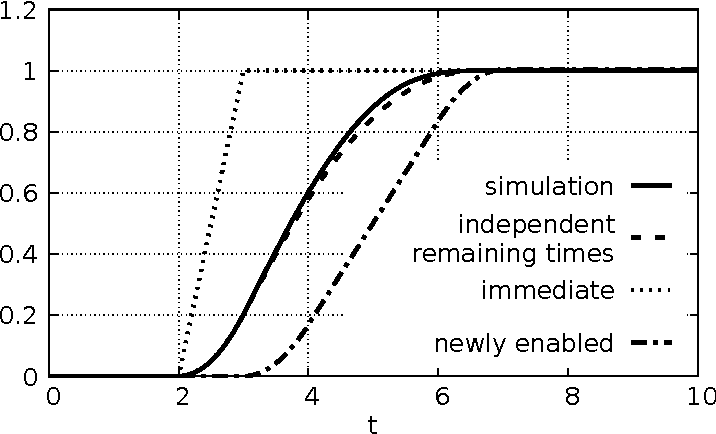
\includegraphics[scale=0.25]{simple_ttd_cdf}}
        \end{center}
      \end{minipage}
      \begin{minipage}{0.3\textwidth}
        \begin{center}
          {\tiny $F_{TTI(1,\omega)}$}\\
          \colorbox{white}{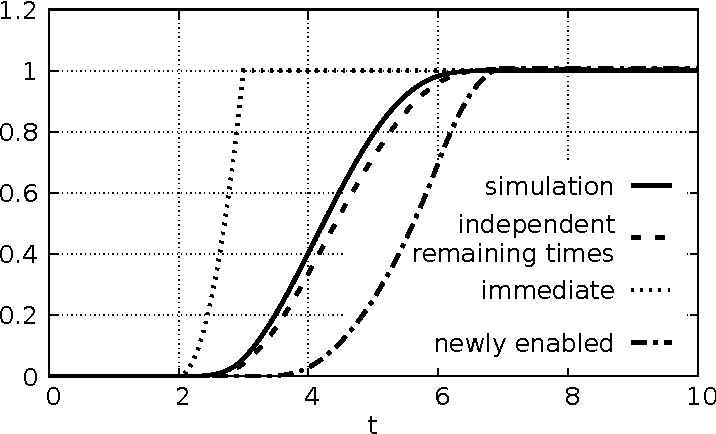
\includegraphics[scale=0.25]{simple_tti_cdf}}
        \end{center}
      \end{minipage}
      \begin{minipage}{0.3\textwidth}
        \begin{center}
          {\tiny $F_{TTSN(2,\omega)}$}\\
          \colorbox{white}{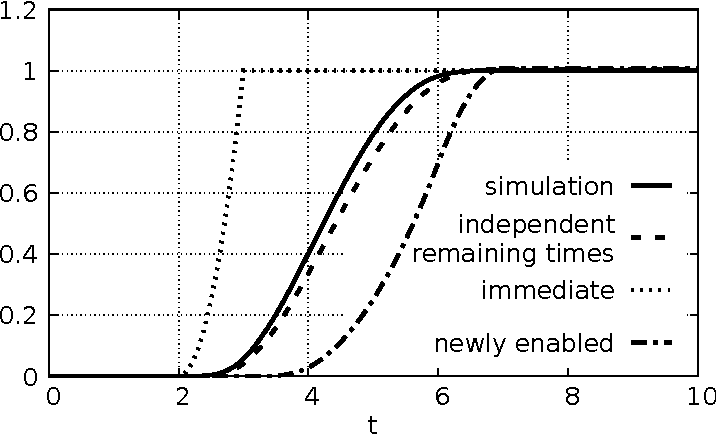
\includegraphics[scale=0.25]{simple_ttsn_cdf}}
        \end{center}
      \end{minipage}
      
      \begin{minipage}{0.5\textwidth}
        \textit{TTD}, \textit{TTI} and \textit{TTSN} computed in
        \begin{itemize}
          \item 41/45/42 min for simulation
          \item 0.15/0.18/0.10 s for bounds
        \end{itemize}
      \end{minipage}
      \begin{minipage}{0.45\textwidth}
        \vspace{2em}
        Very good approximation results
        \begin{itemize}
          \item especially for \textit{independent remaining times}
        \end{itemize}
        Feasible approach
        \begin{itemize}
          \item very fast bounds evaluation
          \item compared to simulation
        \end{itemize}
      \end{minipage}
    \end{frame}
    
    \begin{frame}{Complex assembly line}{TTDone, TTIdle, TTStartNext}
      \begin{minipage}{0.3\textwidth}
        \begin{center}
          {\tiny $F_{TTD(5,\omega)}$}\\
          \colorbox{white}{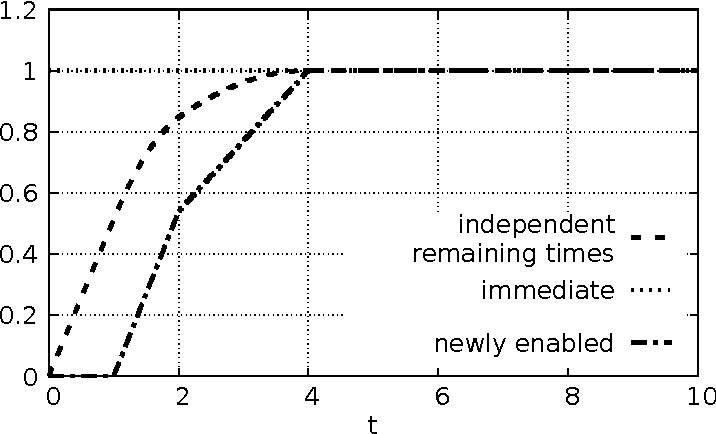
\includegraphics[scale=0.25]{complex_ttd_cdf}}
        \end{center}
      \end{minipage}
      \begin{minipage}{0.3\textwidth}
        \begin{center}
          {\tiny $F_{TTI(5,\omega)}$}\\
          \colorbox{white}{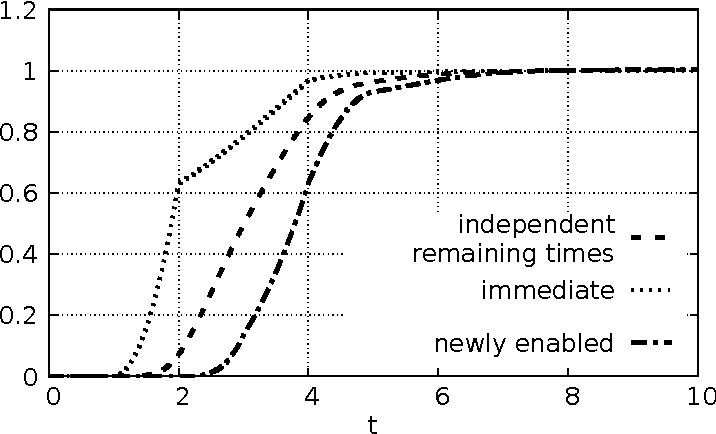
\includegraphics[scale=0.25]{complex_tti_cdf}}
        \end{center}
      \end{minipage}
      \begin{minipage}{0.3\textwidth}
        \begin{center}
          {\tiny $F_{TTSN(5,\omega)}$}\\
          \colorbox{white}{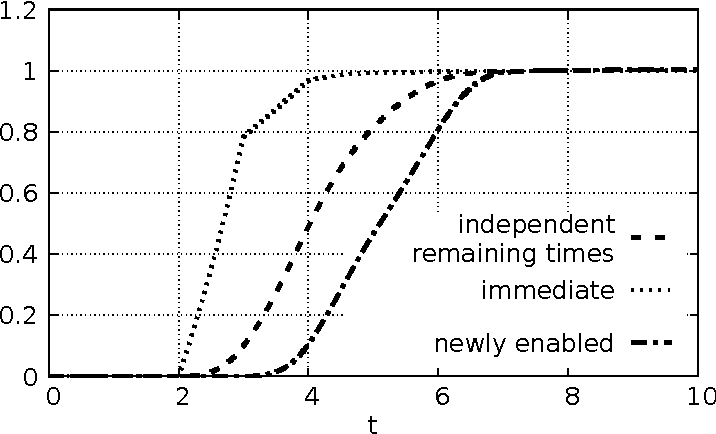
\includegraphics[scale=0.25]{complex_ttsn_cdf}}
        \end{center}
      \end{minipage}
      
      \vspace{4em}
      \begin{minipage}{0.5\textwidth}
        \textit{TTD}, \textit{TTI} and \textit{TTSN} computed in
        \begin{itemize}
          \item 0.126/0.123/0.75 s for bounds
        \end{itemize}
      \end{minipage}
      \begin{minipage}{0.45\textwidth}
        Scalable solution
        \begin{itemize}
          \item in a complex scenario
          \item simulation would be infeasible
        \end{itemize}
      \end{minipage}
    \end{frame}
